\section{Staged experiment (II articls)}


Devices with a gliding arc are classified according
to power supply regime as <<\textbf{bipolar}>> and \textbf{unipolar}>>.
In the bipolar regime of power supply, sign-alternating 
sinusoidal voltage is applied to two electrodes of a
device.

In this experiment and ours, we work with a Flyback transformer, so that the signal is rectified in the unipolar case.

\begin{figure}[h]
    \centering
    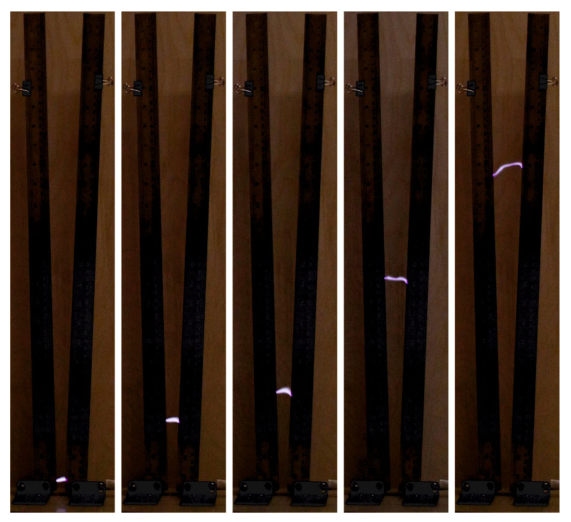
\includegraphics[width=0.3\textwidth]{figures/1.png}
    \caption{Experiment for Article II.}
\end{figure}

It was founded, that it moves with a constant velocity on most of the path. Also, the the dependence of the arc rise speed on the angle between the electrodes was investigated.

